
\section{Ultrasound Design Gallery}\label{section:method}

\subsection{User Interface of \usdg}\label{section:ui}

\begin{figure}[th]
  \centering
  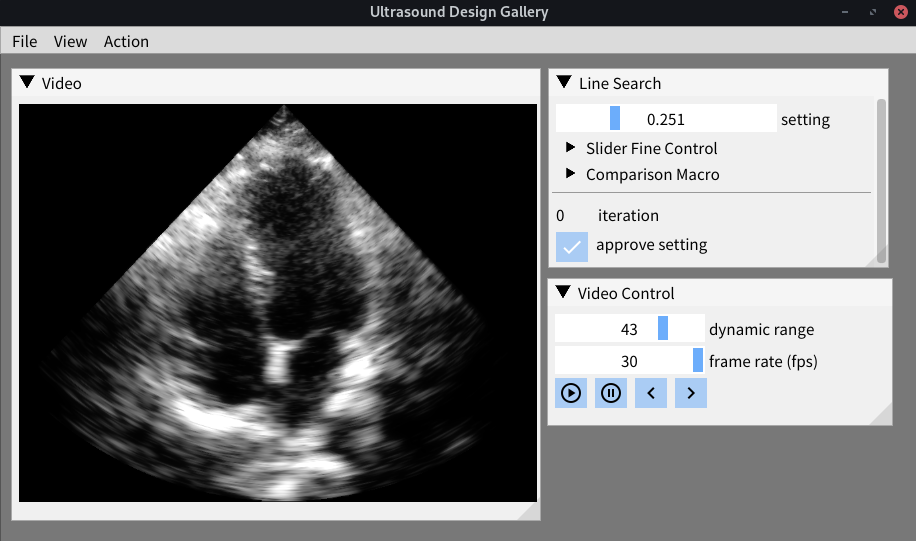
\includegraphics[scale=0.35]{figures/ui.png}
  \caption{User interface of the Ultrasound Design Gallery}
\end{figure}

\begin{figure}[th]
  \centering
  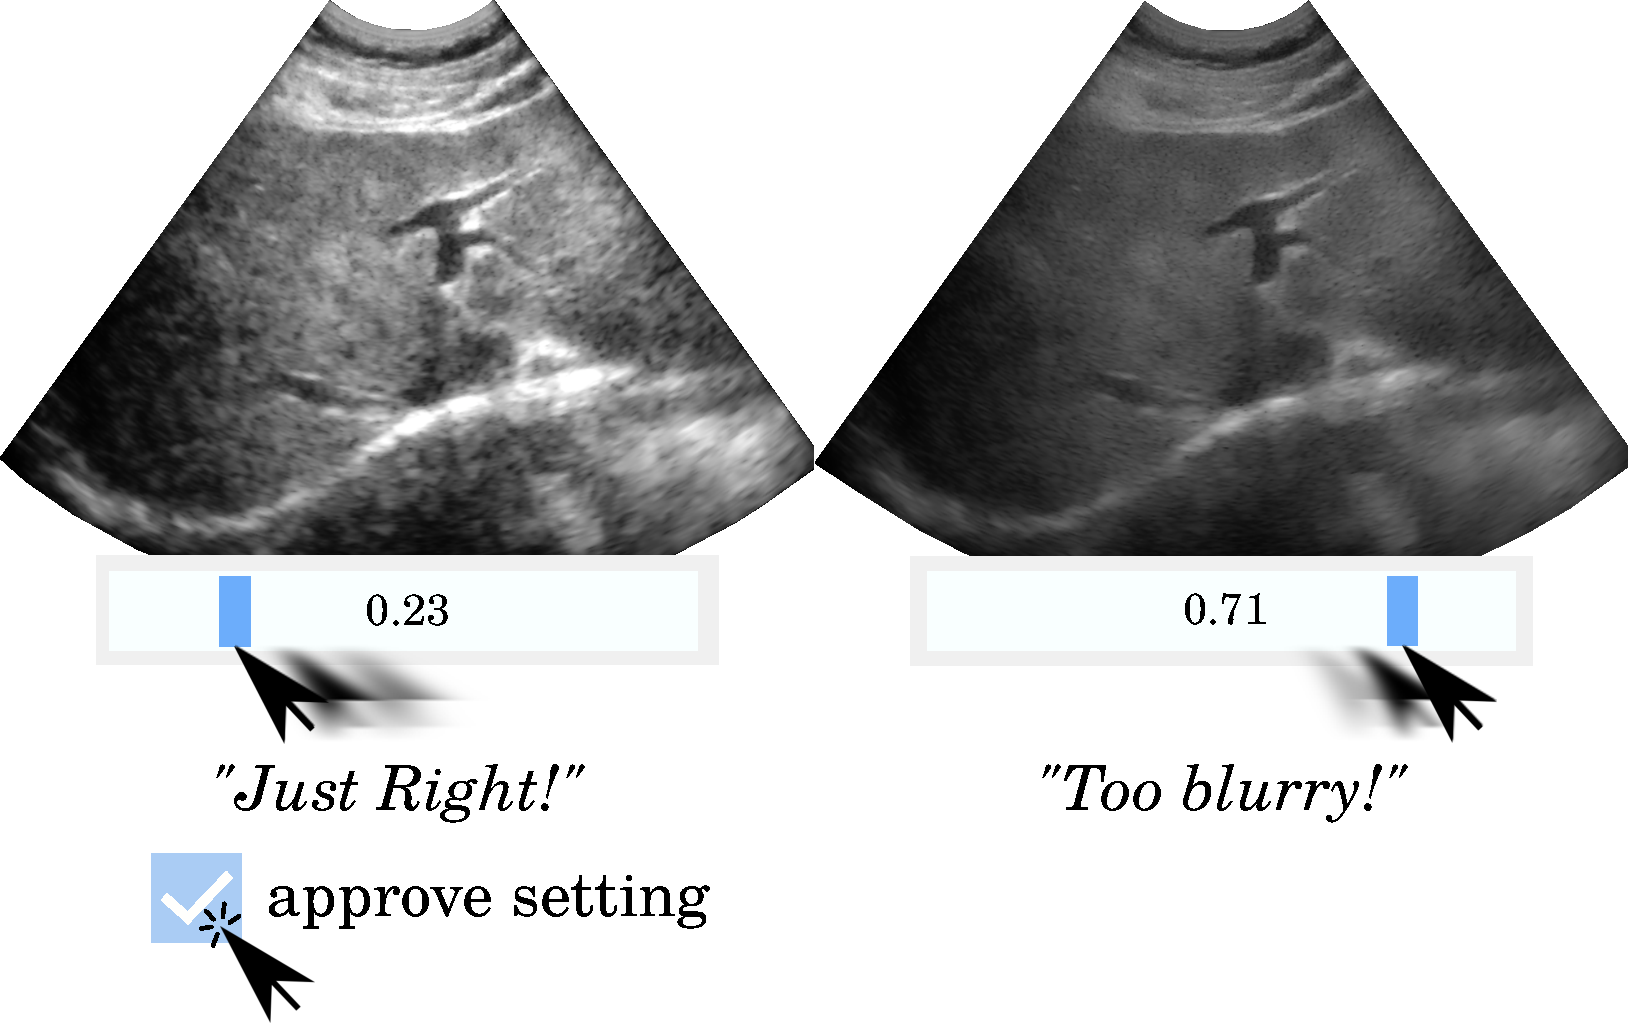
\includegraphics[scale=0.35]{figures/ui_interaction.pdf}
  \caption{Visualization of the interaction with the Ultrasound Design Gallery}
\end{figure}

\begin{figure}[th]
  \centering
  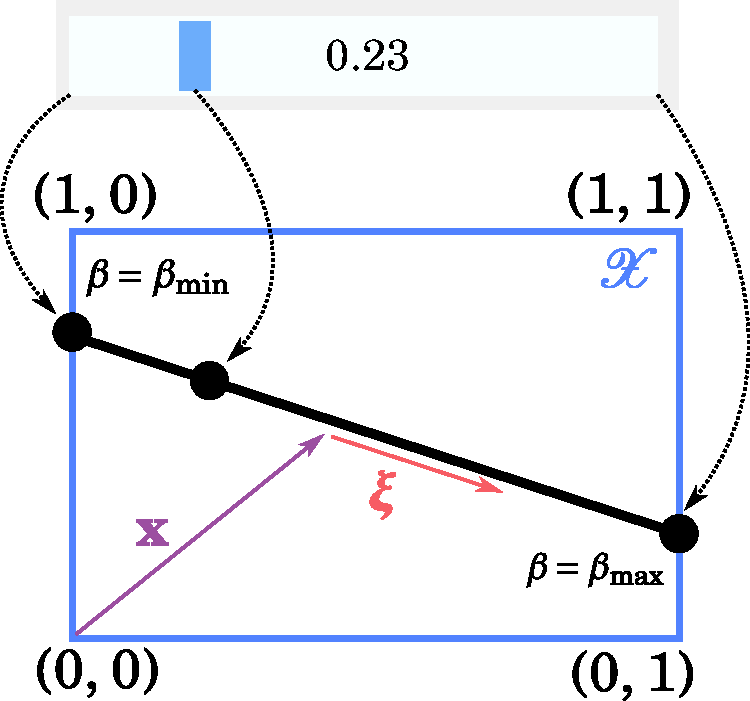
\includegraphics[scale=0.45]{figures/linesearch.pdf}
  \caption{}
\end{figure}

\subsection{Learning {\user}s Preference with Gaussian Processes}\label{section:gp}

\subsubsection{Probabilistic Model}
Recently, Mikkola \textit{et al.} showed a clever formulation~\cite{pmlr-v119-mikkola20a}.
\begin{align*}
\epsilon_{\vf}           &\sim p\,(\epsilon_{\vf}) \\
\sigma                  &\sim p\,(\sigma) \\
\vf \mid \epsilon_{\vf}  &\sim \mathcal{GP}(0, \mK + \epsilon_{\vf}^2\mI) \\
  f(\alpha\,\vxi + \vx) > f(\beta_i \,\vxi + \vx) \mid \vf,\, \sigma
  &\sim p\,(\alpha,\, \beta_i,\, \vx,\,\vxi,\, \mid \epsilon,\, \vf)  \\
\end{align*}

\begin{figure}[t]
  \removelatexerror
  \begin{algorithm2e}[H]
    \DontPrintSemicolon
    \SetAlgoLined
    \KwIn{Precomputed Cholesky decomposition of \(\mK\),
      convergence criterion, 
      gradient function of the likelihood \(\nabla_{\vf}\, p(\mathcal{D}\mid\vf)\),
      Hessian function of the joint \(\nabla^2_{\vf}\, p(\mathcal{D},\, \vf)\).
    }
    \KwOut{
      \(\vf_{t}\), \(\mW_t\).
    }
    \( \vf_1 \leftarrow \mathbf{0} \)\;
    \Repeat{ until convergence } {
      \(\valpha        \leftarrow \mK\backslash\vf_{t} \)\;
      \(\vg            \leftarrow \nabla_{\vf}\, p(\mathcal{D}\mid\vf)|_{\vf = \vf_t} - \valpha \)\;
      \(\mW_t          \leftarrow -  \nabla^2_{\vf}\, p(\mathcal{D},\, \vf) \)\;
      \(\mB           \leftarrow \mI + \mK \mW \)\;
      \(\mL_{\mB}, \mU_{\mB} \leftarrow \mathrm{lu}\,(\mB) \)\;
      \(\vp           \leftarrow \mL_{\mB} \backslash \mU_{\mB} \backslash \mK \vg \)\;
      \(\vf_{t+1}      \leftarrow \vf_t + \eta \, \vp \)\;
      \(t \leftarrow t + 1\)\;
    }
    \caption{Newton's Method for Laplace's Approximation}\label{alg:newton}
  \end{algorithm2e}
\end{figure}
%
\subsubsection{Laplace's Approximation}
We approximate the posterior \(p\,(\vf\,|\,\vtheta,\, \mathcal{D})\) with Laplace's approximation~\cite{williams_bayesian_1998}.
Laplace's approximation performs a second order Taylor expansion around the maximum of the posterior such that
\begin{align}
q\,(\vf) = \mathcal{N}\left(\vf;\, \vf^*,\, {(\mK^{-1} + \mW)}^{-1}\right) \approx p\,(\vf \mid \vtheta,\, \mathcal{D})
\end{align}
where \(\vf^*\) is the maximum a-posteriori estimate such that \(\nabla_{\vf}\, p\,(\mathcal{D},\, \vf)|_{\vf = \vf^*} = 0\), \(\mW = -\nabla^2_{\vf}\, p\,(\mathcal{D},\,\vf)|_{\vf=\vf^*} \) is the negative Hessian of the likelihood at \(\vf^*\), and \(\mK\) is the covariance matrix.
In general, \(\mH\), the Hessian of \(p\,(\mathcal{D},\vf)\) turns out structured.
This allows efficient implementations of Newton's method for finding \(\vf^*\).
For example,~\cite{rasmussen_gaussian_2006} discusses cases where \(\mH\) is diagonal or block-diagonal.
Unfortunately, in our case, the structure of \(\mH\) is neither.
We thus provide a different implementation of Newton's iteration that uses the identities
\begin{align}
  {\big(\mK^{-1} + \mW\big)}^{-1}
  &= {\Big(\mK^{-1} \big(\mI + \mK \mW \big)\Big)}^{-1} \\
  &= {{\big(\mI + \mK \mW \big)}^{-1} \mK} \\
  &= \mB^{-1} \mK \\
  &= \mU_{\mB}^{-1} \, \mL_{\mB}^{-1} \, \mK \label{eq:BinvK}
\;.
\end{align}
where \cref{eq:BinvK} is computed using the LU decomposition of \(\mB\) and back-substitution.
A detailed illustration is provided in~\cref{alg:newton} where \(\vp\) is the Newton direction, the stepsize \(\eta\) is found using backtracking line search with Armijo's condition~\cite{nocedal_numerical_2006}.

\subsubsection{Predictive Distribution}
For prediction, we use a formulation of \({\big(\mK^{-1} + \mW\big)}^{-1}\) different from~\cref{eq:BinvK}.
This is because the variance prediction \(\sigma^2(\vx)\) which requires to compute a inverse quadratic term \(\mK^{\top}(\vx) {\big(\mK^{-1} + \mW\big)}^{-1} \vk(\vx)\), which can be efficiently computed when a Cholesky decomposition of \(\mL_{\mathcal{L}} \, \mL^{-1}_{\mathcal{L}}  = {\big(\mK^{-1} + \mW\big)}\) is available.
The formulation of~\cref{eq:BinvK} does not directly provide a closed form expression for the Cholesky.
We thus use the indentities
\begin{align}
  {\big(\mK^{-1} + \mW\big)}^{-1}
  &= { \Big({\big(\mL\,\mL^{\top}\big)}^{-1} + \mW \Big) }^{-1} \label{eq:Kcholid}  \\
  &= { \big(\mL^{-\top}\,\mL^{-1} + \mW \big) }^{-1}  \\
  &= { \Big( \mL^{-\top}\,\big(\mI + \mL^{\top}\,\mW\,\mL \big)\,\mL^{-1} \Big) }^{-1}  \\
  &= \mL\,{\big(\mI + \mL^{\top}\,\mW\,\mL \big)}^{-1}\,\mL^{\top}  \\
  &= \mL\, \mC^{-1} \,\mL^{\top}  \\
  &= \big( \mL\, \mL_{\mC}^{-1} \big)\, {\big( \mL\, \mL_{\mC}^{-1} \big)}^{\top} \label{eq:Ccholid} \\
  &= \mL_{\mathcal{L}} \, { \mL_{\mathcal{L}} }^{\top}
\end{align}
where~\cref{eq:Kcholid} uses the precomputed Cholesky decomposition of \(\mK\) and~\cref{eq:Ccholid} requires the Cholesky decomposition of \(\mC = \mI + \mL^{\top}\,\mW\,\mL\).

The GP prediction using \(q\,(\vf)\) are computed as
\begin{align}
  \mu\,(\vx)
  &= {\vk(\vx)}^{\top} \mK^{-1} \, \vf^*  \\
  \sigma^2\,(\vx)
  &= k(\vx, \vx) - \vk^{\top}(\vx) \, {(\mK^{-1} + \mW)}^{-1} \, \vk(\vx) \\
  &= k(\vx, \vx) - {\big( \mL_{\mathcal{L}} \vk(\vx) \big)}^2
\end{align}

\subsubsection{Hyperparameter Treatment}
While previous works observed that the full Bayesian approach improves performance~\cite{henrandez-lobato_predictive_2014, snoek_practical_2012}, recent experimental results suggest that such performance improvement may not be significant~\cite{ath_bayesian_2021}.
In our case, the exact marginal likelihood is not available.
Thus, full Bayesian inference requires pseudo-marginal MCMC~\cite{filippone_pseudomarginal_2014, pmlr-v51-murray16} methods, which suffer from low statistical effieciency for high-dimensions.
Also, the real-time nature of our application makes the use of these methods very delicate in terms of computational efficiency and robustness.
We experimented with full Bayesian inference using pseudo-marginal slice-sampling~\cite{pmlr-v51-murray16} and concluded that it is not worth the computational cost.

Some theoretical~\cite{berkenkamp_noregret_2019} and practical~\cite{wang_adaptive_2013} works have suggested that expert tuned hyperparameters achieve better performance than full Bayesian treatments.

%% \paragraph{Pseudo-Marginal MCMC}
%% Using our approximation \(q\,(\vf)\), we use  for sampling both \(\vf\) and \(\vtheta\) from the posterior.
%% The marignal likelihood is approximated using importance sampling such that
%% \begin{align}
%%   \tilde{p}\,(\mathcal{D}\mid\theta)
%%   &= \int p\,(\mathcal{D}\mid\vf)\,p\,(\vf\mid\vtheta) d\vf \\
%%   &\approx \frac{1}{N_{\mathrm{pm}}} \sum^{N_{\mathrm{pm}}}_{i=1} \frac{p\,(\mathcal{D}\mid\vf_i)\,p\,(\vf_i\mid\vtheta)}{q\,(\vf_i)}
%% \end{align}
%% where \(\vf_i\) are samples from \(q\,(\vf)\) and \(N_{\mathrm{pm}}\) is the number of samples.
%% For simplicity, we use the maximum a-posteriori estimate \(\vf^*\).

%% For sampling \(\theta\) and \(\sigma\), we use elliptical slice sampling~\cite{murray_elliptical_2010}.
%% To resolve this problem, Murray \& Graham propose pseudo-marginal slice sampling~\cite{}.

%% Using the ARD hyperparameters alone for sensitivity analysis results is not very effective~\cite{pmlr-v89-paananen19a}.
%% Also, the non-identifiability of ARD hyperparameters complicates their statistical analysis~\cite{zhang_inconsistent_2004a}.
%% ARD is severely affected by dimensionality.
%% This manifests as low acceptance rates in MCMC procedures~\cite{filippone_pseudomarginal_2014}.

\subsection{Optimizing \User~Preference with Preferential Bayesian Optimization}\label{section:bo}

\begin{align}
 &\minimize_{\vx,\, \vxi}\;\; a\,(\vx, \vxi \mid \mathcal{D}) \\
 &\text{subject to}\;\; \vx \in \mathcal{X},\; \norm{\vxi}_{\infty} = 1
\end{align}

Given \(\vx_t\) and \(\vxi_t\), the user is expected to solve the line-search problem
\begin{align}
 \alpha = &\argmax_{ \beta }\; f\,(\beta\,\vxi + \vx) \\
 &\text{subject to}\;\; \beta_{\text{min}} \leq \beta \leq \beta_{\text{max}}\;.
\end{align}

For binary discrete comparisons, the \textit{expected improvement} (EI) acquisition function~\cite{jones_efficient_1998} defined as
\begin{align}
  a_{\mathrm{EI}}(\vx) = \Esub{ y \sim \mathcal{N}(\mu(\vx),\, \sigma^{2}(\vx)) }{ \max\big(\, y - y^*, 0 \,\big) }
\end{align}
where \(y^* = \argmax_{\vx} \mu\,(\vx) \), has been commonly used~\cite{NIPS2007_b6a1085a}.
In our case, the fact that \(\vx\) and \(\vxi\) form a \textit{line} complicates the use of EI.

\subsubsection{Approximate Expected Improvement}
\cite{10.1145/3072959.3073598} proposed to formulate EI as
\begin{align}
  a\,(\vx, \vxi)
  = \mathbb{E}\,\Big[\, \max\big(\, \max\,\big\{\; f\,(\,\beta \xi + \vx\,) \mid \beta \in \mathcal{I} \;\big\}, 0 \,\big)\,\Big],
\end{align}
which is approximated using discrete thompson sampling (DTS) such as
\begin{align}
  &a_{\mathrm{AEI}}\,(\vx, \vxi) 
  = \frac{1}{N_{\mathrm{mc}}} \sum_{j=1}^{N_{\mathrm{mc}}} \max\,(\, \max\,\big\{\; y_i, \ldots, y_{N_\beta} \;\big\}, 0 \,) \label{eq:aei} \\
  &\text{where} \;\;  \beta_i \sim p\,(\beta), \nonumber\\
  &\quad\qquad y_i \sim \mathcal{N}\big( \mu\,(\,\beta_i \vxi + \vx \,),\, \sigma^2\,(\, \beta_i \vxi + \vx \,) \big).\nonumber
\end{align}
The outer expectation is approximated using a Monte Carlo average and \(y_i\) are the DTS samples generated from the GP predictive distribution.
We will call the DTS realization \textit{approximate EI} (AEI).

Computing gradients of AEI (whether stochastic or not) is in general challenging.
The original implementation of~\cite{pmlr-v119-mikkola20a} thus approximates the gradients using finite-difference and used L-BFGS for optimization.
However, since the gradients approximated using~\cref{eq:aei} are \textit{stochastic}, the use of L-BFGS can be tricky depending implementation details.
For example, line-search schemes commonly used in L-BFGS can easily fail with noisy objective functions.
Instead, we use the stochastic approximation simultaneous perturbation (SPSA,~\cite{spall_overview_1998, spall_implementation_1998}) which is a more principled method for using noisy finite-difference apprroximations.
Fundamentally, SPSA is a stochastic gradient descent method where the gradients are approximated using finite-difference.

\subsubsection{Hybrid Expected Improvement Schemes}
The stochastic nature of AEI may negatively affect the resolution of the solutions.
We therefore consider a more deterministic scheme
\begin{align}
  \vx_t  &= \argmax_{\vx}  a_{\mathrm{EI}}(\vx) \\
  \vxi_t &= \argmax_{\vxi} a_{\mathrm{AEI}}(\vx_t, \vxi) \label{eq:hei_xi}
\end{align}
which is a hybrid of vanilla EI and AEI.
For solving~\cref{eq:hei_xi}, we use random search~\cite{karnopp_random_1963} by evaluating AEI on samples from the \(L\)-\(\infty\) hypersphere.
Our hybrid EI (HEI) scheme has two advantages:
\begin{enumerate}
\item The exact gradient \(a_{\mathrm{EI}}(\vx)\) is available.
  This enables the use of L-BFGS for finding \(\vx\) with high fidelity.
\item The line \(\mathcal{I}\) formed by \(\vx_t, \xi_t\) always includes the point optimal with respect to vanilla EI.
\end{enumerate}

\subsubsection{Expected Improvement with Koyama's Scheme}
Facing a similar problem, Koyama et al. used a heuristic scheme where
\begin{align}
  \vx_t   &= \argmax_{\vx} a_{\mathrm{EI}}(\vx) \\
  \vx^*   &= \argmax_{\vx} \mu\,(\vx) \\
  \vxi_t  &=  \frac{\vx_t - \vx^*}{\norm{ \vx_t - \vx^* }_{\infty}}.
\end{align}
That is, they chose to interpolate between the EI point and the currently best known solution.

\subsection{Image Enhancement Method}
Laplacian pyramid method~\cite{zhang_multiscale_2006, zhang_nonlinear_2007, kang_new_2016}.

%
\begin{tikzpicture}
  % Place nodes using a matrix
  \matrix (m1) [row sep=2.0mm, column sep=3.0mm]
{
    \node[dspnodeopen] (input)  {\textit{input}}; &
    \node[coordinate] ()       {};       &
    \node[coordinate] ()        {};      &
    \node[coordinate] ()        {};      &
    \node[coordinate] ()       {};       &
    \node[coordinate] ()        {};      &
    \node[dspnodeopen] (output)  {\textit{output}};   \\
%
    \node[coordinate] (G0in) {};          &
    \node[dspnodefull,dsp/label=below] (G0)  {\(G_0\)};   &
    \node[dspadder,label=278:\(-\)]    (L0j)   {};          &
    \node[dspnodefull] (L0)    {\(L_0\)};   & 
    \node[dspfilter, text width=1.3cm]  (diff0) {denoise}; &
    \node[dspfilter, text width=2.2cm]  (edge0) {edge enhance}; &
    \node[dspadder]    (out0j)   {};  \\
%
    \node[dspsquare]  (dcm1)  {\downsamplertext{2}}; &
    \node[coordinate] ()      {};          &
    \node[dspsquare]  (itp1)  {\upsamplertext{2}}; &
    \node[coordinate] ()       {};          &
    \node[coordinate] ()        {};          &
    \node[coordinate] ()        {};          &
    \node[dspsquare]  (outitp1) {\upsamplertext{2}}; \\
%
    \node[coordinate] (dcm1out)  {}; &
    \node[coordinate] ()      {};          &
    \node[coordinate] (dcm1out2) {}; \\
%%
    \node[coordinate]  (dcm1out3)    {};   &
    \node[dspnodefull,dsp/label=below] (G1)    {\(G_1\)};   &
    \node[dspadder,label=278:\(-\)]    (L1j)   {};          &
    \node[dspnodefull] (L1)    {\(L_1\)};   & 
    \node[dspfilter, text width=1.3cm]  (diff1) {denoise}; &
    \node[dspfilter, text width=2.2cm]  (edge1) {edge enhance}; &
    \node[dspadder]    (out1j)   {};  \\
%
    \node[dspsquare]  (dcm2)  {\downsamplertext{2}}; &
    \node[coordinate] ()      {};          &
    \node[dspsquare]  (itp2)  {\upsamplertext{2}}; &
    \node[coordinate] ()       {};          &
    \node[coordinate] ()        {};          &
    \node[coordinate] ()        {};          &
    \node[dspsquare]  (outitp2) {\upsamplertext{2}}; \\
%
    \node[coordinate] (dcm2out)  {}; &
    \node[coordinate] ()      {};          &
    \node[coordinate] (dcm2out2) {}; \\
%%
    \node[coordinate]  (dcm2out3)    {};   &
    \node[dspnodefull,dsp/label=below] (G2)    {\(G_2\)};   &
    \node[dspadder,label=278:\(-\)]    (L2j)   {};          &
    \node[dspnodefull] (L2)    {\(L_2\)};   & 
    \node[dspfilter, text width=1.3cm]  (diff2) {denoise}; &
    \node[dspfilter, text width=2.2cm]  (edge2) {edge enhance}; &
    \node[dspadder]    (out2j)   {};  \\
%
    \node[dspsquare]  (dcm3)   {\downsamplertext{2}}; &
    \node[coordinate] ()       {};          &
    \node[dspsquare]  (itp3)   {\upsamplertext{2}}; &
    \node[coordinate] ()       {};          &
    \node[coordinate] ()       {};          &
    \node[coordinate] ()        {};          &
    \node[dspsquare]  (outitp3) {\upsamplertext{2}}; \\
%
    \node[coordinate] (dcm3out)  {}; &
    \node[coordinate] ()      {};    &
    \node[coordinate] (dcm3out2) {}; \\
%%
    \node[coordinate]  (dcm3out3)    {};   &
    \node[dspnodefull,dsp/label=below] (G3)    {\(G_3\)};   &
    \node[coordinate] (L3j)   {};          &
    \node[coordinate] (L3)    {};   & 
    \node[dspfilter, text width=1.3cm]  (diff3) {denoise}; &
    \node[dspfilter, text width=2.7cm]  (edge3) {contrast enhance}; &
    \node[coordinate]  (out3) {e}; \\
  };

  \begin{scope}[start chain]
    \chainin (G0in);
    \chainin (G0)    [join=by dspline];
    \chainin (L0j)   [join=by dspconn];
    \chainin (L0)    [join=by dspline];
    \chainin (diff0) [join=by dspconn];
    \chainin (edge0) [join=by dspconn];
    \chainin (out0j) [join=by dspconn];
  \end{scope}

  \begin{scope}[start chain]
    \chainin (dcm1out3);
    \chainin (G1)    [join=by dspline];
    \chainin (L1j)   [join=by dspconn];
    \chainin (L1)    [join=by dspline];
    \chainin (diff1) [join=by dspconn];
    \chainin (edge1) [join=by dspconn];
    \chainin (out1j) [join=by dspconn];
  \end{scope}

  \begin{scope}[start chain]
    \chainin (dcm2out3);
    \chainin (G2)      [join=by dspline];
    \chainin (L2j)     [join=by dspconn];
    \chainin (L2)      [join=by dspline];
    \chainin (diff2)   [join=by dspconn];
    \chainin (edge2)   [join=by dspconn];
    \chainin (out2j)   [join=by dspconn];
  \end{scope}

  \begin{scope}[start chain]
    \chainin (dcm3out3);
    \chainin (G3)    [join=by dspline];
    \chainin (L3j)   [join=by dspline];
    \chainin (L3)    [join=by dspline];
    \chainin (diff3) [join=by dspconn];
    \chainin (edge3) [join=by dspconn];
    \chainin (out3)  [join=by dspline];
  \end{scope}
  %%

  \begin{scope}[start chain]
    \chainin (dcm1out);
    \chainin (dcm1out2) [join=by dspline];
    \chainin (itp1)     [join=by dspconn];
    \chainin (L0j)      [join=by dspconn];
  \end{scope}

  \begin{scope}[start chain]
    \chainin (dcm2out);
    \chainin (dcm2out2) [join=by dspline];
    \chainin (itp2)     [join=by dspconn];
    \chainin (L1j)      [join=by dspconn];
  \end{scope}

  \begin{scope}[start chain]
    \chainin (dcm3out);
    \chainin (dcm3out2) [join=by dspline];
    \chainin (itp3)     [join=by dspconn];
    \chainin (L2j)      [join=by dspconn];
  \end{scope}

  %%

  \begin{scope}[start chain]
    \chainin (input);
    \chainin (G0in)     [join=by dspline];
    \chainin (dcm1)     [join=by dspconn];
    \chainin (dcm1out3) [join=by dspline];
    \chainin (dcm2)     [join=by dspconn];
    \chainin (dcm2out3) [join=by dspline];
    \chainin (dcm3)     [join=by dspconn];
    \chainin (dcm3out3) [join=by dspline];
  \end{scope}

  \begin{scope}[start chain]
    \chainin (out3);
    \chainin (outitp3) [join=by dspconn];
    \chainin (out2j)   [join=by dspconn];
    \chainin (outitp2) [join=by dspconn];
    \chainin (out1j)   [join=by dspconn];
    \chainin (outitp1) [join=by dspconn];
    \chainin (out0j)   [join=by dspconn];
    \chainin (output)  [join=by dspconn];
  \end{scope}
\end{tikzpicture}


%%% Local Variables:
%%% TeX-master: "master"
%%% End:

\begin{figure*}
  \centering
  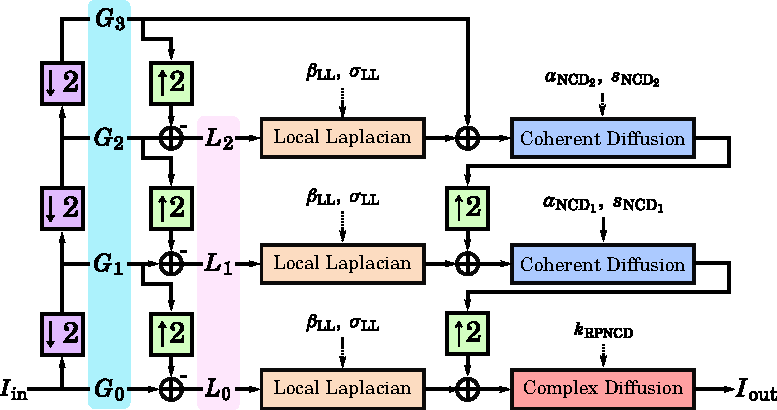
\includegraphics[scale=1.0]{figures/multiscale_filter.pdf}
  \caption{}
\end{figure*}

%%% Local Variables:
%%% TeX-master: "master"
%%% End:
